\documentclass[11pt,twocolumn]{article}
\usepackage[utf8]{inputenc}
\usepackage[english]{babel}
\usepackage{pdfpages}
\usepackage{hyperref}

\usepackage{verbatim}

\title{Network Analysis in ArangoDB}
\date{January 2020}
\author{Alessandro d'Agostino, Mattia Ceccarelli, Riccardo Scheda}

\begin{document}

\twocolumn[
\begin{@twocolumnfalse}

\maketitle

\begin{abstract}
The project aim is to develop a simple python API that let the user interact with the open-source multi-model database ArangoDB to perform fast queries on multi-partite graphs, extract and visualize sub-network which can then be analized with powerful python libraries.
The study also includes results on the computational efficiency of ArangoDB's algorithms, in order to have an estimate of the API timing behaviours with large networks.
\end{abstract}
\end{@twocolumnfalse}
]

\section{Introduction}
ArangoDB \cite{WEBSITE:arangodb} is a multi-model, open-source database with flexible data models for documents, graphs and key-values. It is being used in different fields: from semantic analysis to genome studies.

In the present work we employed the library \verb python-arango  \cite{WEBSITE:pythonarango} to import and export multipartite network-like databases, that are defined as collections of documents (nodes) and collections of relationships between them (edges).

In particular, a document is a python dictionary with a mandatory \verb _id  key assigned to a unique value.
What we call an "edge" is also a python dictionary, but with an \verb _id , \verb _source  and \verb _target  voices, to specify not only the linked nodes, but also the direction of said link in the case of directed graphs.

\paragraph{Graph Object}
A Graph is the combination of at least one node collection and one or multiple edge collections, called edge definitions.
With a Graph two main operations are available: visualization and execution of queries.

The former is possible thanks to ArangoDB web interface, as shown in the figures below, which provide the user many options such as the starting node and the number of elements to load. By default, the starting node is random.

For the latter we relied on the poweful AQL, that is the query language implemented in arango. It is used to execute different kind of "search" through the graph, and select nodes and edges.

\paragraph{Why ArangoDB?}
ArangoDB resulted to be the NoQL engine with the most favorable compromise between memory usage and computation speed among others available alternatives. (CHIEDERE TABELLA CON LE PRESTAZIONI A NICO)
ArangoDB offers a valid web interface where all the commands could be given intuitively and graph and queries' results could be visualized in an organic way.
Furthermore there are several ArangoDB Python interfaces available on line, which allowed us to taylor this poweful tool to our needs.

\paragraph{NetworkX}
Even though ArangoDb allows fast queries it is necessary the right tool to study the characteristics of a resulting subnet.Forthis purpose we decided to exploit mainly the Python library NetworkX \cite{WEBSITE:networkx} due to its huge availability of function and tools.

\section{Pipeline}
Now we describe a typical usage case and all the operations needed to extract a subgraph in ArangoDB.
The first thing to do is to read the file in the right input format (typically \texttt{.gexf}) through the function \texttt{read\_gexf}:

\begin{verbatim}
read_gexf(db,
          filename,
          nodes_collection_name='nodes',
          edges_collection_name='edges',
          graph_name='Net')
\end{verbatim}

The funcion takes the information about nodes and edges from the gexf file and creates the corrispondent  collections on the ArangoDB engine. Then it returns two graphs: one python-arango type and one of networkx type.

Once that the graph and the collections of nodes and edges are uploaded on Arango web interface we can proceede with futher analysis. For instance we can perform a graph traversal aimed to extract the first neighbours of a certain node.

In this case we can make use of python-arango, calling the function:

\begin{verbatim}
first_neighbours = traverse(db,
         starting_node,
         nodes_collection_name,
         graph_name,
         direction='outbound',
         item_order='forward',
         min_depth=0,
         max_depth=1,
         vertex_uniqueness='global')
\end{verbatim}

Tuning the given parameters actually every traversal could be performed. The ouput of this type of function is meant to be the resulting sub net saved as Python dictionaries containing vertex and the path crossed by the traverse.

Having the list of the first neighbours we can obtain the corresponding subnet just using the function \texttt{subgraph} given by Networkx:

\begin{verbatim}
Nx_Sub_Net =
        Nx_Net.subgraph([vertex['label']
        for vertex in
        first_neighbours['vertices']])
\end{verbatim}

In this way we create the minimal subgraph containing only with the labels of nodes and the corresponding edges. To recover the whole information contained in the starting network we add all the attributes back to each node:

\begin{verbatim}
for node in Nx_Sub_Net:
      attr = pa.get_vertex(db,
                           {'label':node},
                           'Sym_Deas')
      nx.set_node_attributes(Nx_Sub_Net,
                     {node : attr})
\end{verbatim}

The last thing to do is to import the subnet in ArangoDB, using the two specific functions  \texttt{nx\_to\_arango} and \texttt{eport\_to\_arango}:


\begin{verbatim}
sub_net = nx.readwrite.node_link_data(Nx_Sub_Net)
sub_net = pa.nx_to_arango(sub_net, 'Sub_Net')
Sub_Net = pa.export_to_arango(db,
                  sub_net ,
                  'Sub_Net',
                  'Sub_Net_edges',
                  'Sub_Graph')
\end{verbatim}

Now the resulting subnet is ready for every kind of analysis offered by NetworkX. This is a usefull procedure to extract articulated subnet even on big non-relational base. Managing a huge amount of information is in fact one of the weak points of a straight NetworkX build.



\section{Timing}
As just mentioned one of the main focuses is to apply queris to very big networks.Therefore a study on how the time spent to perform a query scales with the increase in dimension of the network under analysis was necessary. Hence we detected three different traversals to be performed on several graphs with similar characteristics but different dimensions.

We created random graphs with a number of nodes ranging from 100 to 10000, using the NetworkX function \texttt{fast\_gnp\_random\_graph}. Then we runned the queries under study onto 10 different graphs for each number of nodes, in order to obtain an average value and an idea of its dispersion. The plots of one of theese time series is reported below in
Figure \ref{fig:1}.

\begin{figure}[ht]
  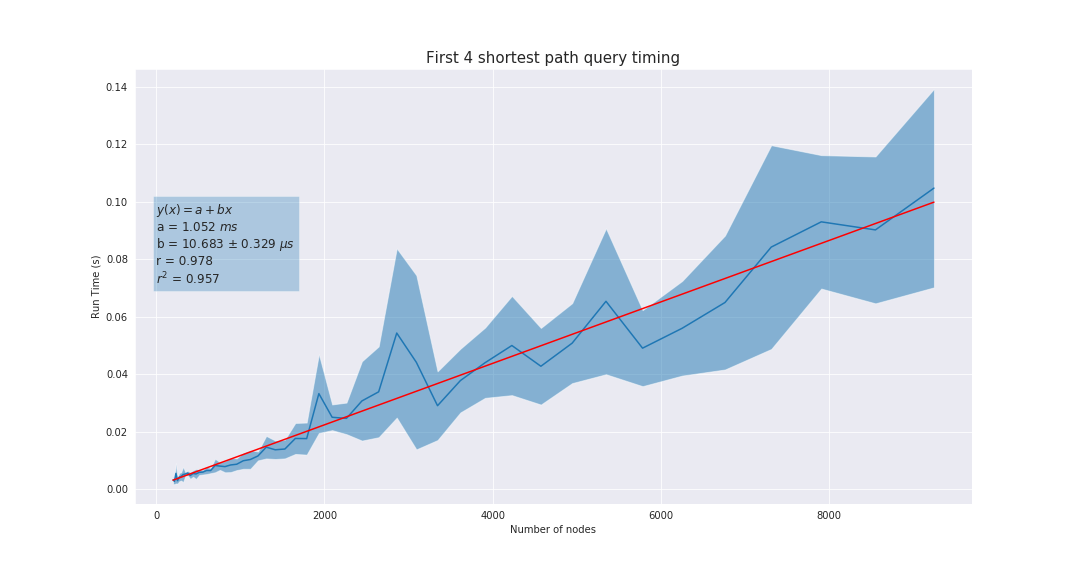
\includegraphics[width=\linewidth]{images/4_shortest_path_timing.png}
  \caption{\small{\textit{Boccaccio: "Times"}}}
  \label{fig:1}
\end{figure}

We performed a linear fitting on the sampled data and a quite linear relationship emerged in each case, with an R$^2$ coefficient always $ \geq 0.9$. From this analysis we can extrapolate the behaviour facing an arbitrary big network dimension [Express better this concept]

[Does it worth to mention the "exponential" sampling technique? I think we could overfly on it.]

\section{Results}

\section{Conclusions}

We've produced an applicative to visualize and efficiently query a graph-like database with a simple yet resourceful programming language like python.

As shown in the results, the scaling of the ArangoDB query algorithm is linear for the two cases taken into consideration, k shortest path and neighborood search. This is promising for future application in large dataset.

\paragraph{Problems}

The main problems lie in the level of control we can gather through python. Indeed, it seems to be impossible to load and save default queries.
Moreover, we couldn't manage to save graph visualization options, which could ease the accessibility.

\paragraph{Future Ideas}

We will focus on preparing the applicative for the non-programmer user.

We think a Graphical User Interface (GUI) could greatly smoothen the user experience.

In the future we want to test the applicative with a much larger database than the one we had at disposal.

\twocolumn[
\begin{@twocolumnfalse}
\bibliography{biblio}
\bibliographystyle{ieeetr}
\end{@twocolumnfalse}
]

\end{document}
